%%This is a very basic article template.
%%There is just one section and two subsections.
\documentclass[a4paper, 11pt]{article}
\usepackage[pdftex]{graphicx}
\usepackage{parskip}
\usepackage{hyperref}
\usepackage[all]{hypcap}
\usepackage{amsmath}
\usepackage{amsfonts}
\usepackage{xcolor}
\usepackage{enumitem}
\usepackage{adjustbox}

\title{Assignment 4 \\ Math 205 Linear Algebra}
\author{Syed Ammar Mahdi \\sm03691 \and Muhammad Shahzain \\ms03977 \and Muhammad Shahrom Ali \\ma03559}


\newcommand{\mat}[1]{\boldsymbol { \mathsf{#1}} }
\newcommand{\MYhref}[3][blue]{\href{#2}{\color{#1}{#3}}}


\begin{document}
\setlength{\parskip}{10pt} % 1ex plus 0.5ex minus 0.2ex}
\setlength{\parindent}{0pt}
\DeclareGraphicsExtensions{.pdf,.png,.gif,.jpg}
\maketitle

\section*{Solutions}
\begin{enumerate} 


\item You are given two functions:
\begin{align}
f(x,y) &= -1 + 4(e^x - x) - 5x\sin y + 6y^2 \\
g(x,y) &= (x^2 - 2x)\cos y
\end{align}

Determine whether $(0, 0)$ and $(1, \pi)$ is the stationary point for $f(x,y)$ and $g(x,y)$ respectively. If they are the stationary points, then determine the nature of the stationary points

%Q1
\textbf{Solution:}



\item Using the quadratic form $\vec x^T \mat A \vec x$, show that $f(x, y) = x^2 + 4xy + 3y^2$ does not have a minimum at $(0, 0)$

%Q2
\textbf{Solution:}


\item Let $\mat A = \begin{bmatrix} 1 & b & 0 \\ c & 4 & 2 \\ 0 & 2 & 4 \end{bmatrix}$. For what values of $b$ and $c$, the matrix will be positive definite and positive semi-definite?

%Q3
\textbf{Solution:}


\item Determine whether the following statements are true or false. You must give counterexamples and/or justifications for your choice

%Q4

\begin{enumerate}
    \item Given 
        $
        \mat{A} = 
        \begin{bmatrix}
        a_1 & a_2 \\
        a_3 & a_4
        \end{bmatrix}$  and 
        $
        \mat{B} = \;
        \begin{bmatrix}
        b_1 & b_2 \\
        b_3 & b_4
        \end{bmatrix}$, then the following equation holds
        $\mat{AB} - \mat{BA} = \mat{I}$ (where $\mat{I}$ is the identity matrix).
    %Test AM & GM
	
\textbf{Solution:}

    \item The matrix 
        $\begin{bmatrix}
        a & b \\
        0 & a
        \end{bmatrix}$ is diagonalizable 

	\textbf{Solution:}
\end{enumerate}        

\item Let $ \Vec{p}, \Vec{q} \in \mathbb R^{n}$. If $ \mat{A} = \Vec{p} \Vec{q}^{T}$

%Q5

a.) Show that $\Vec{p}$ is an eigenvector and find it's corresponding eigenvalue $\lambda$. 

\textbf{Solution:}

b.) Determine all the other eigenvalues of $\mat{A}$ and explain how you obtained them.

\textbf{Solution:}

c.) What can you say about the trace of $\mat{A}$?

\textbf{Solution:}

\item The great barrier reef has been known to include over 1500 species of fish. One particular fish that is indigenous to that area is the clown fish. Data shows that in the first year 4000 clown fish inside the reef migrated to other areas, while 2250 clown fish migrated to the reef. It is estimated that the ratio of clown fish leaving the reef to the population inside the reef is constant. Similarly, the ratio of clown fish entering the reef to the population outside the reef is also constant. With an initial population of 22500 clown fish outside the reef and 20000 clown fish inside the reef, construct a system that is indicative of the number of fish inside (as well as outside) after the end of the first year. 

Will the system ever reach a steady state? If so, approximately how long would it take to reach such a state? How will this state be affected if the initial population values were doubled? 

You will be given points for clear and concise explanations.

%Q6
\textbf{Solution:}


\item It just so happens that we have lost all the data that you had submitted for assignment 3. The question now arises as to how we are supposed to grade this assignment. The TAs have suggested that we use a formula where the grade for each assignment (from the third onwards) will be calculated by taking the average of the previous two (i.e. $A_3 = \frac{1}{2}*(A_2+A_1) $.  

%Q7

a.) Find the matrix $\mat{B}$ such that the following system is satisfied:

$
\begin{bmatrix}
A_{k+2}\\
A_{k+1}
\end{bmatrix} = \mat{B} \;
\begin{bmatrix}
A_{k+1}\\
A_{k}
\end{bmatrix}
$
where $k \geq 1$ 
\newline

\textbf{Solution:}

b.) Find the eigenvalues and eigenvectors of $\mat{B}$.

\textbf{Solution:}

c.) Find the limit as $n \rightarrow \infty$ of the matrices $\mat{B^n} = S \Lambda ^{n}S^{-1}$.

\textbf{Solution:}

\item
%Q8

%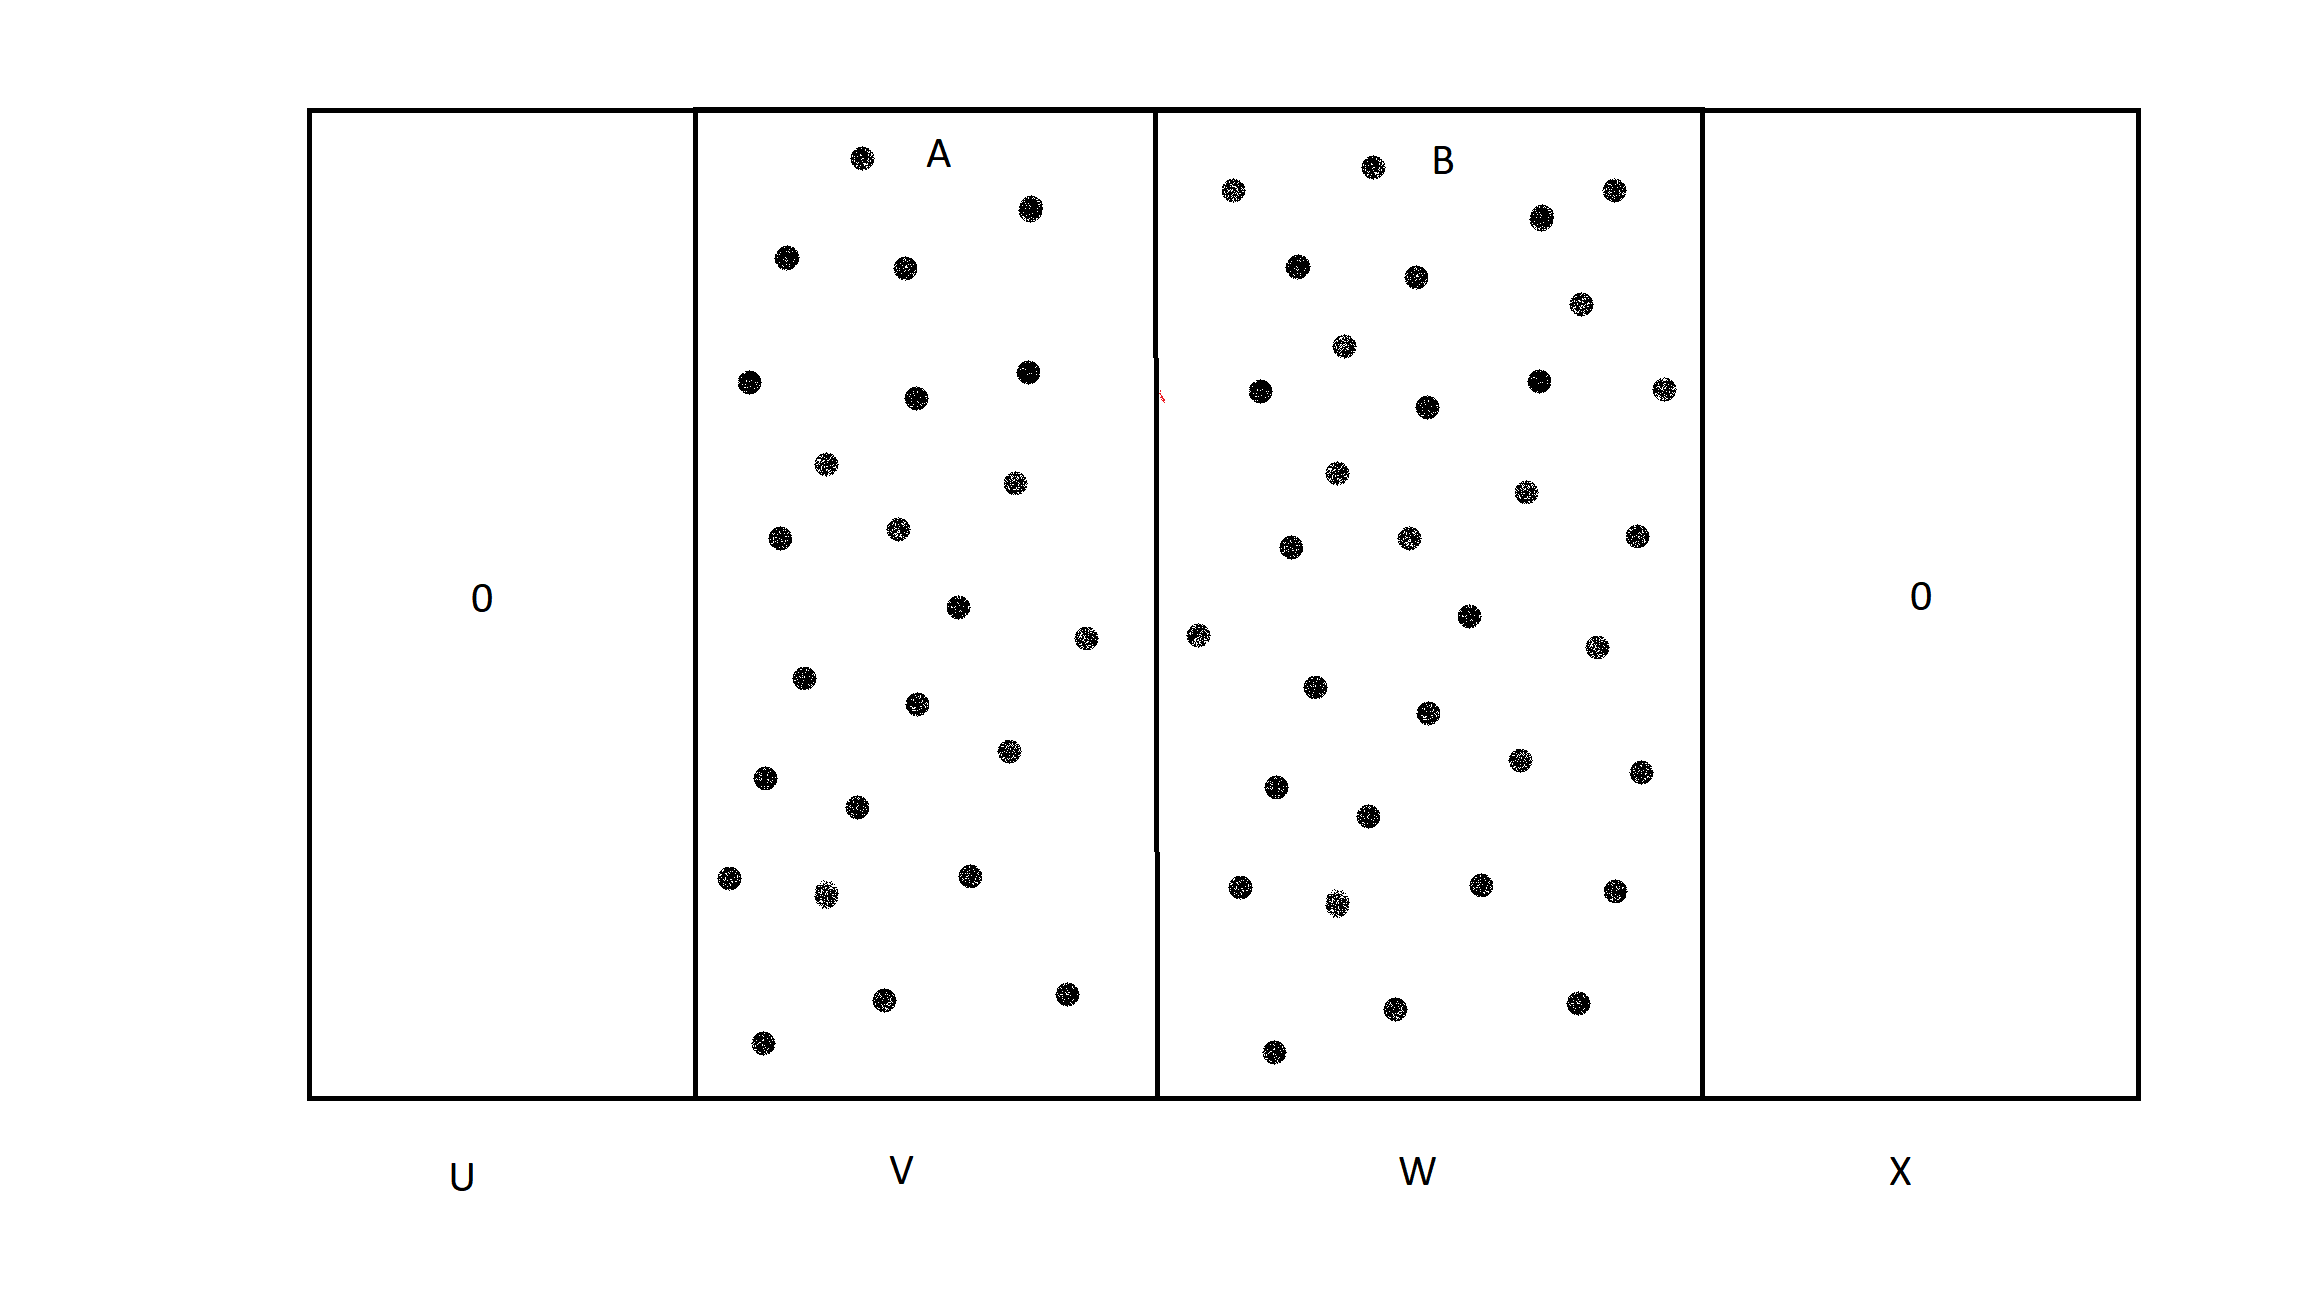
\includegraphics[width=\textwidth]{figs/Diffusion.png}
\adjustbox{valign=t}{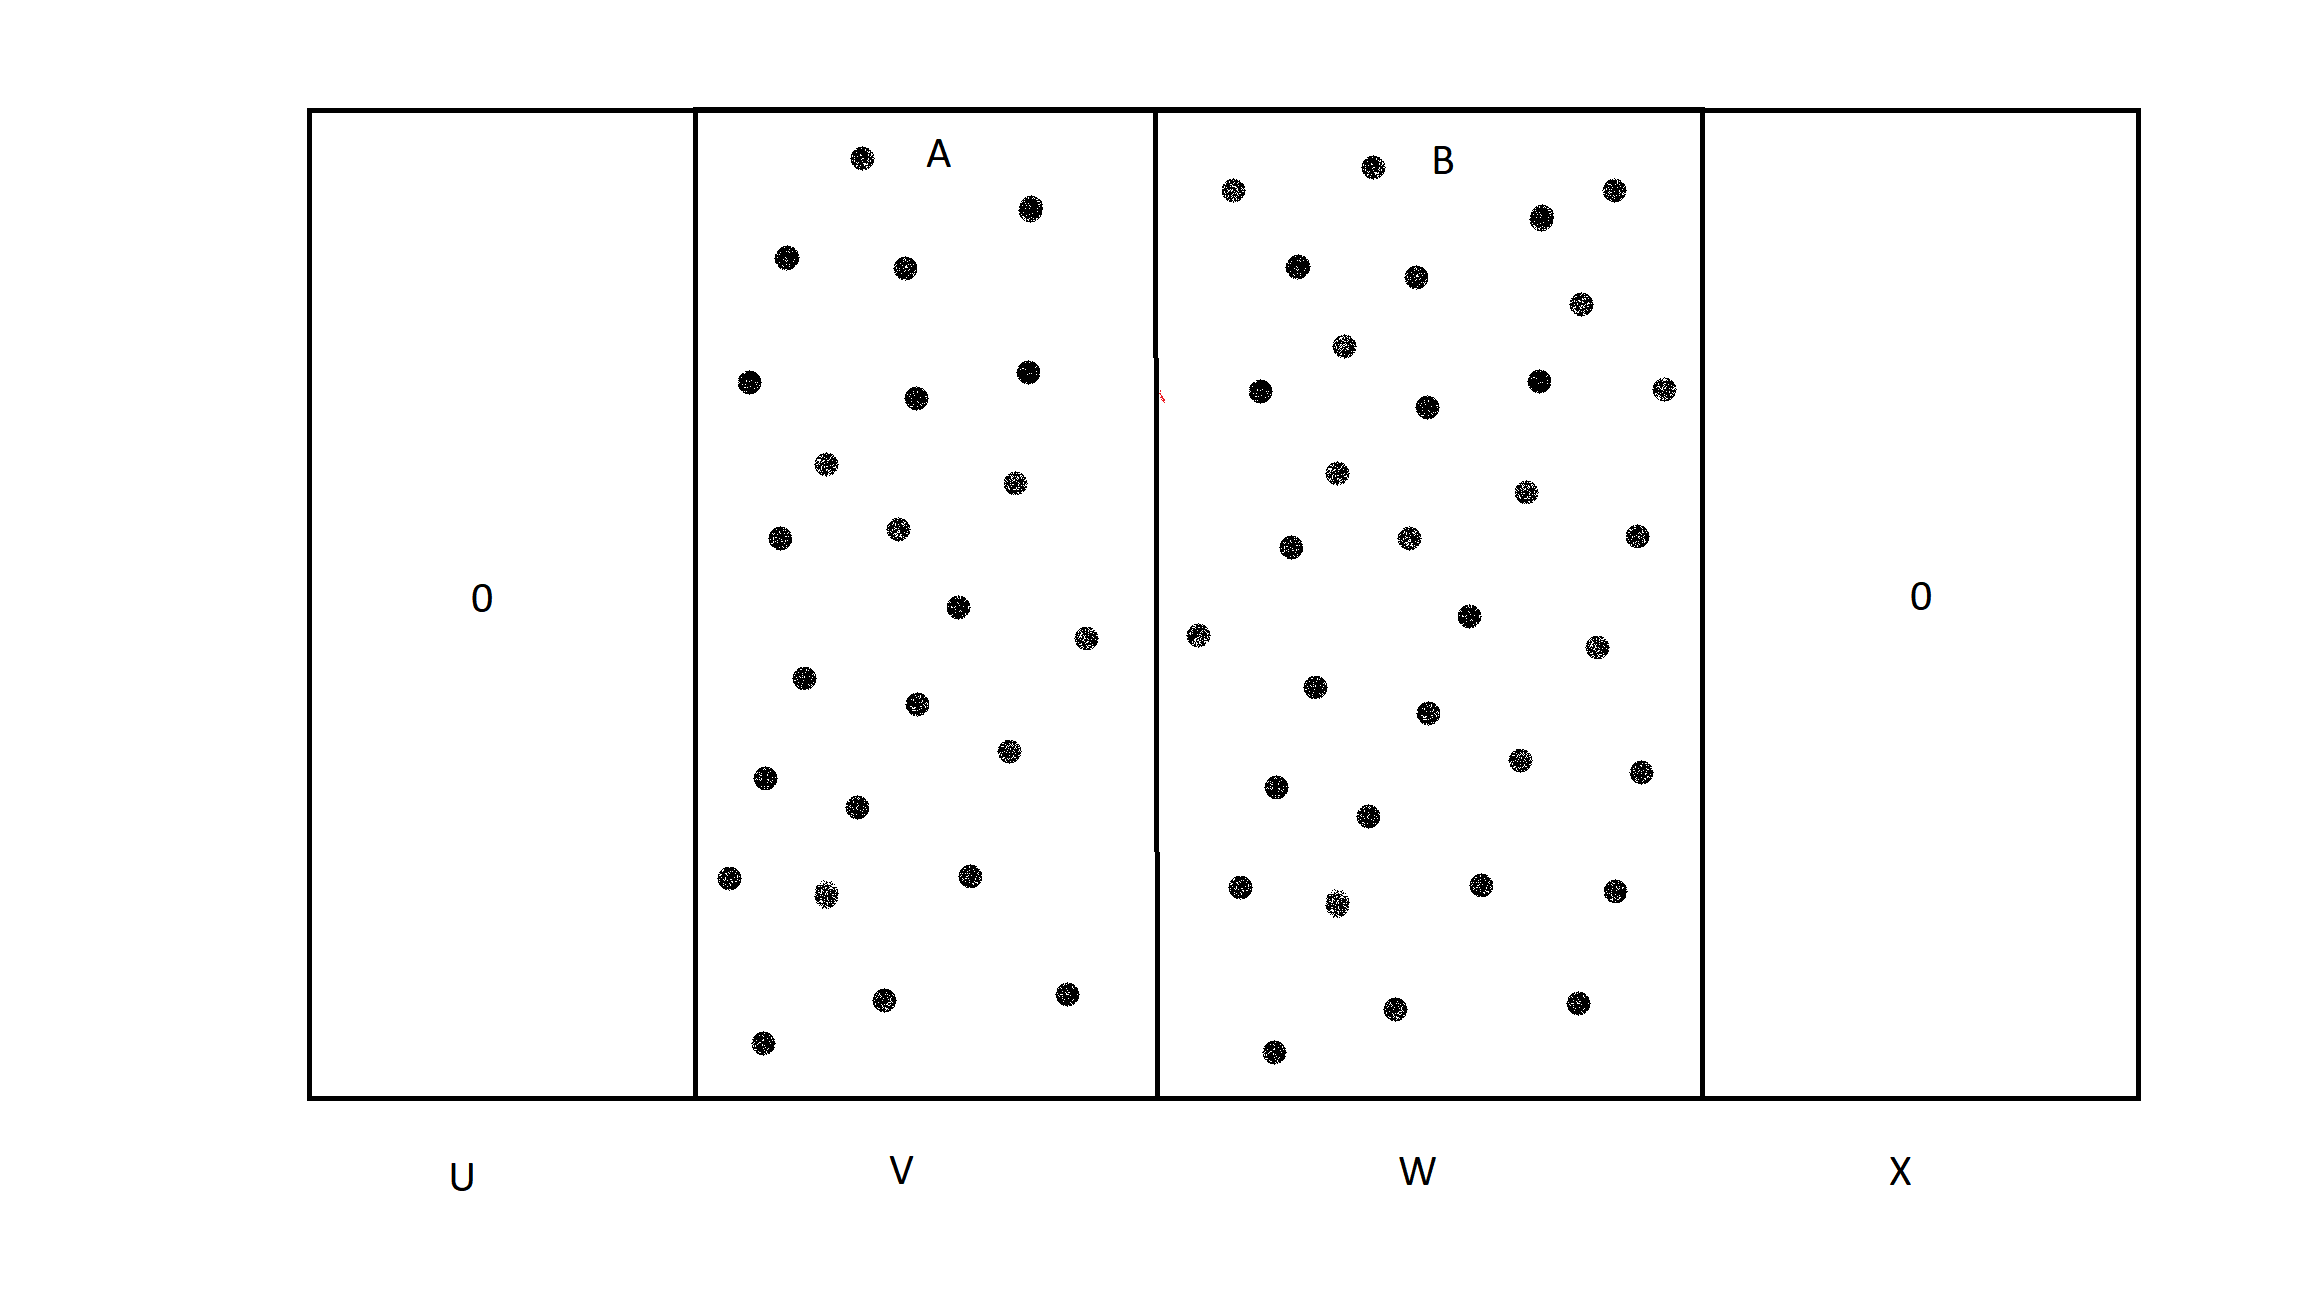
\includegraphics[width=\textwidth]{figs/Diffusion.png}}
The figure above shows a room that has been divided into 4 parts u,v,w and x. Initially, sections v and w contain gas with concentrations $A$ and $B$ respectively. At each unit of time, the gas in sections $v$ and $w$ diffuses to it's adjacent sections at a rate that is equal to the difference in concentrations of the respective sections. You may assume that within a section the gas is uniformly spread.

a.) Construct a system that involves the rate of flow into $v$ and the rate of flow into $w$.

\textbf{Solution:}

b.) Determine the rate at which the concentrations decay.

\textbf{Solution:}

c.) What happens to the concentrations as $t \rightarrow \infty$

\textbf{Solution:}

\end{enumerate}

\newpage

\section*{Appendix A:}

\newpage

\begin{thebibliography}{}
\end{thebibliography}

\end{document}